\documentclass[noauthor,nooutcomes]{ximera}

\usepackage{todonotes}

\renewcommand{\alt}[1]{\ensuremath{\vadjust{\todo{#1}}}}

\makeatletter
\define@key{answer}{alt}{}
\makeatother

\let\image\relax
\let\endimage\relax
\NewEnviron{image}{
  \begin{center}\BODY\end{center}% center
}

\colorlet{textColor}{black}
\colorlet{background}{white}
\colorlet{penColor}{blue!50!black} % Color of a curve in a plot
\colorlet{penColor2}{red!50!black}% Color of a curve in a plot
\colorlet{penColor3}{red!50!blue} % Color of a curve in a plot
\colorlet{penColor4}{green!50!black} % Color of a curve in a plot
\colorlet{penColor5}{orange!80!black} % Color of a curve in a plot
\colorlet{penColor6}{yellow!70!black} % Color of a curve in a plot
\colorlet{fill1}{penColor!20} % Color of fill in a plot
\colorlet{fill2}{penColor2!20} % Color of fill in a plot
\colorlet{fillp}{fill1} % Color of positive area
\colorlet{filln}{penColor2!20} % Color of negative area
\colorlet{fill3}{penColor3!20} % Fill
\colorlet{fill4}{penColor4!20} % Fill
\colorlet{fill5}{penColor5!20} % Fill
\colorlet{gridColor}{gray!50} % Color of grid in a plot




\title{Assignment}
\begin{document}
\begin{abstract}
\end{abstract}
\maketitle

\section{Calculus}

\begin{problem}
  Compute the derivative of $f(x) = 3x^2 + 2x - 5 %% Math mode defaults to mathml, prompt is read.
  \begin{prompt}f'(x) = \answer{6x + 2}%% \answer comes in with built in default \alt{answer}
  \end{prompt}$.
\end{problem}

\section{Finance}

Here we do a finance question.

\subsection{A problem}


\begin{question}
  When you take out a loan, the amount of the loan is called
  \textbf{principal}.  For most loans, interest is calculated monthly,
  based on an \textbf{annual interest rate}, and based on the remaining
  balance.  When you make a payment, your payment first offsets the
  accumulated interest and then is applied to principal, in order to
  calculate the \textbf{remaining principal balance}.  The loan is paid
  back in full when the remaining principal balance is reduced to zero.
  
  Suppose you borrow $\$5,000$ and agree to pay it back in equal
  annual payments over $5$ years.  Interest is calculated at $7\%$,
  compounded annually.  We will approach this problem numerically.
  Use your guess for the annual payment, and complete the table
  below. Round all answers to the nearest cent.
  \[ 
  \alt{ A loan pay-off table showing the 0th year in the first row,
    followed by the first year in the second row, followed by the
    second year in the third row, the third year in the fourth row,
    and the fifth year in the sixth row.  The first column is the
    year, the second column is the interest, the third column is the
    balance with interest, the fourth column is the payment, the fifth
    column is the remaining principal balance.}
  \begin{array}{|c|c|c|c|c|}
   \hline
   \text{Year} & \text{Interest}             & \text{Balance with Interest} & \text{Payment}    & \text{Remaining Principal Balance}\\ \hline
   0  & \$ 0               & ---        & \$ 0     & \$ 5000 \\ \hline
   1  & \$ \answer[alt={interest in the first year}, tolerance=0]{350} & \$ \answer[alt={balance with interest in the first year},tolerance=0]{5350}& \$ 1250\alt{payment in the first year is \$1250}  & \$ \answer[alt={remaining principal balance in the first year},tolerance=0]{4100} \\ \hline
   2  & \$ \answer[alt={interest in the second year}, tolerance=0]{287}& \$ \answer[alt={balance with interest in the second year},tolerance=0]{4387}    & \$ 1250\alt{payment in the second year is \$1250}  & \$ \answer[alt={remaining principal balance in the second year},tolerance=0]{3137} \\ \hline
   3  & \$ \answer[alt={interest in the third year},tolerance=0]{219.59} & \$ \answer[alt={balance with interest in the third year},tolerance=0]{3356.59} & \$ 1250\alt{payment in the third year is \$1250} & \$ \answer[alt={remaining principal balance in the third year},tolerance=0]{2106.59} \\ \hline
   4  & \$ \answer[alt={interest in the fourth year},tolerance=0]{147.46} & \$ \answer[alt={balance with interest in the fourth year},tolerance=0]{2254.05} & \$ 1250\alt{payment in the fourth year is \$1250}  & \$ \answer[alt={remaining principal balance in the fourth year},tolerance=0]{1004.05} \\ \hline
   5  & \$ \answer[alt={interest in the fifth year},tolerance=0]{70.28}  & \$ \answer[alt={balance with interest in the fifth year},tolerance=0]{1074.33} & \$ 1250\alt{payment in the fifth year is \$1250} & \$ \answer[alt={remaining principal balance in the fifth year},tolerance=0]{-175.67} \\ \hline
 \end{array}
 \]
\end{question}

\section{A worked example}

\begin{example}
Sketch the graph of the function defined by $f(x)=2x^3-3x^2-12x$.

The $y$-intercept is $(0,\answer[given]{0})$. Place this point on your plot.

\begin{image}\alt{We show the $(x,y)$ plane with a point plotted at the origin.}
\begin{tikzpicture}
	\begin{axis}[
            domain=-2:4,
            xmin=-2,
            xmax=4,
            ymax=25,
            ymin=-25,
            axis lines =middle, xlabel=$x$, ylabel=$y$,
            every axis y label/.style={at=(current axis.above origin),anchor=south},
            every axis x label/.style={at=(current axis.right of origin),anchor=west}
          ]
         \addplot[color=penColor,fill=penColor,only marks,mark=*] coordinates{(0,0)};  %% closed hole
        \end{axis}
\end{tikzpicture}
%% \caption{We start by placing the point $(0,0)$.}
%\label{figure:CS1}
\end{image}



Which of the following are vertical asymptotes?  Select all that apply.

\begin{selectAll}%% This should render automatically as checkboxes
	\choice{$x=0$}
	\choice{$x=1$}
	\choice{$x=-1$}
	\choice{$x=\sqrt{2}$}
	\choice[correct]{There are no vertical asymptotes}
\end{selectAll}

In this case, $f(x) =2x^3-3x^2-12x$, we can find the
$x$-intercepts.   There are three $x$ intercepts.  Call them $a$, $b$, and $c$, and order them such that $a<b<c$.  Then

\begin{align*} %% Alt can default to mathml
  a &= \answer[given]{\frac{3-\sqrt{105}}{4}},\\
  b &= \answer[given]{0}, \\
  c &= \answer[given]{\frac{3+\sqrt{105}}{4}}.
\end{align*}



  Which of the following best describes the end behavior of $f$ as $x \to \infty$?		
  \begin{multipleChoice} %% This should render automatically as radiobuttons
    \choice[correct]{$f$  increases without bound.}
    \choice{$f$ decreases without bound.}
    \choice{$f$ has a horizontal asymptote.}
    \choice{$f$ has some other behavior at $\infty$.}
  \end{multipleChoice}
  Which of the following best describes the end behavior of $f$ as $x \to -\infty$?		
  \begin{multipleChoice}
    \choice{$f$  increases without bound.}
    \choice[correct]{$f$ decreases without bound.}
    \choice{$f$ has a horizontal asymptote.}
    \choice{$f$ has some other behavior at $\infty$.}
  \end{multipleChoice}

Compute $f'(x)$ and $f''(x)$,
\begin{align*}
  f'(x) &= \answer[given]{6x^2 -6x -12}\\
  &=6\left(\answer[given]{x^2-x-2}\right)\\
  &=6(x+1)\left(\answer[given]{x-2}\right).
\end{align*}
On the other hand
\begin{align*}
  f''(x) &= \answer[given]{12x-6}\\
  &=12\left(\answer[given]{x-\frac{1}{2}}\right).
\end{align*}
The critical points are where $f'(x) = 0$, thus we need to solve
$6(x+1)(x-2) = 0$ for $x$.  This equation has two solutions.  If we
call them $a$ and $b$, with $a<b$, then what are $a$ and $b$?
\[
a = \answer[given]{-1}\qquad\text{and}\qquad b = \answer[given]{2}.
\]

Mark the critical points $x=2$ and $x=-1$ on your plot. %%BADBAD either or answer would be nice
\begin{image}\alt{We add the critical points $x=-1$ and $x=2$ to the plot with the origin plotted as a point on the curve.}
\begin{tikzpicture}
	\begin{axis}[
            domain=-2:4,
            xmin=-2,
            xmax=4,
            ymax=25,
            ymin=-25,
            axis lines =middle, xlabel=$x$, ylabel=$y$,
            every axis y label/.style={at=(current axis.above origin),anchor=south},
            every axis x label/.style={at=(current axis.right of origin),anchor=west}
          ]
         \addplot [dashed, penColor2] plot coordinates {(-1,-25) (-1,25)}; 
         \addplot [dashed, penColor2] plot coordinates {(2,-25) (2,25)}; 
         \addplot[color=penColor,fill=penColor,only marks,mark=*] coordinates{(0,0)};  %% closed hole
        \end{axis}
\end{tikzpicture}
%\caption{Now we add the critical points $x=-1$ and $x=2$.}
%\label{figure:CS2}
\end{image}
Since $f'(x)=6(x+1)(x-2)$, and both factors $(x+1)$ and $(x-2)$ are
negative for $x<-1$, it follows that $f'(x)>0$, and, therefore, our
function is \wordChoice{\choice[correct]{increasing}
  \choice{decreasing}} on $(-\infty,-1)$.


Similarly, since for $-1<x<2$, $(x+1)>0$ and $(x-2)<0$, the
derivative is negative there, and, therefore, our function is
\wordChoice{\choice{increasing} \choice[correct]{decreasing}} on
$(-1,2)$.



And, for $x>2$, both factors $(x+1)$ and $(x-2)$ are positive, and,
therefore, our function is \wordChoice{\choice[correct]{increasing}\choice{decreasing}} on $(2,\infty)$.
  
Hence $x=-1$, corresponding to the point $(-1,7)$ is a local
\wordChoice{\choice[correct]{maximum} \choice{minimum}} and $x=2$,
corresponding to the point $(2,-20)$ is local
\wordChoice{\choice{maximum} \choice[correct]{minimum}} of
$f(x)$. Identify this on your plot.
\begin{image}
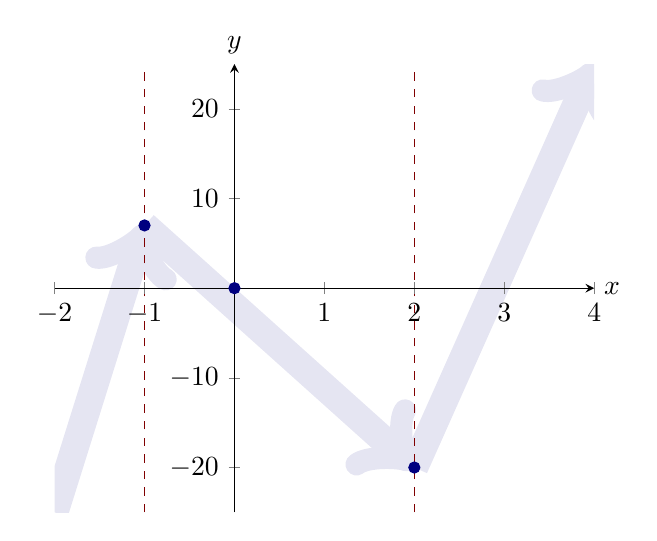
\begin{tikzpicture}
	\begin{axis}[
            axis on top=true,
            domain=-2:4,
            xmin=-2,
            xmax=4,
            ymax=25,
            ymin=-25,
            axis lines =middle, xlabel=$x$, ylabel=$y$,
            every axis y label/.style={at=(current axis.above origin),anchor=south},
            every axis x label/.style={at=(current axis.right of origin),anchor=west}
          ]
          \addplot [->, line width=10, penColor!10!background] plot coordinates {(-2,-25) (-1,7)}; 
          \addplot [->, line width=10, penColor!10!background] plot coordinates {(-1,7) (2,-20)}; 
          \addplot [->, line width=10, penColor!10!background] plot coordinates {(2,-20) (4,25)}; 
          \addplot [dashed, penColor2] plot coordinates {(-1,-25) (-1,25)}; 
          \addplot [dashed, penColor2] plot coordinates {(2,-25) (2,25)}; 
          \addplot [color=penColor,fill=penColor,only marks,mark=*] coordinates{(0,0)};  %% closed hole
          \addplot [color=penColor,fill=penColor,only marks,mark=*] coordinates{(-1,7)};  %% closed hole
          \addplot [color=penColor,fill=penColor,only marks,mark=*] coordinates{(2,-20)};  %% closed hole
          %\addplot [very thick, penColor, samples=100, smooth,domain=(-1.2:-.8)] {2*x^3-3*x^2-12*x};
          %\addplot [very thick, penColor, samples=100, smooth,domain=(1.8:2.2)] {2*x^3-3*x^2-12*x};
        \end{axis}
\end{tikzpicture}
%% \caption{We have identified the local extrema of $f(x)$ and where this
%%   function is increasing and decreasing.}
%% \label{figure:CS3}
\end{image}

In order to locate inflection points, we have to solve the equation $f''(x) = 0$, thus
we need to solve $12\left(x-\frac{1}{2}\right)=0$ for $x$.  

The solution to this is $x = \answer{\frac{1}{2}}$.

This is only a \textbf{possible} inflection point; we still have to check whether concavity changes there.\\

 We have that $f''(x)<0$ for $x<\frac{1}{2}$, therefore
$f$ is concave \wordChoice{\choice{up} \choice[correct]{down}}on $\left(-\infty,\frac{1}{2}\right)$.\\

Similarly, $f''(x)>0$ for $x>\frac{1}{2}$, therefore
$f$ is concave \wordChoice{\choice[correct]{up} \choice{down}} on $\left(\frac{1}{2},\infty\right)$.

So, concavity changes at $x=\frac{1}{2}$, and therefore, this point \wordChoice{\choice[correct]{is} \choice{is not}} a point of inflection.

Since all of this behavior as described above occurs on the interval
$[-2,4]$, we now have a complete sketch of $f(x)$ on this interval,
see the figure below.
\begin{image}
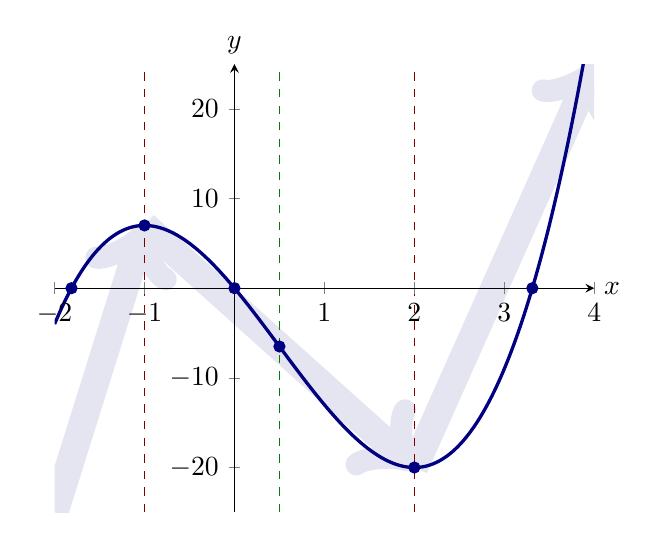
\begin{tikzpicture}
	\begin{axis}[
            axis on top=true,
            domain=-2:4,
            xmin=-2,
            xmax=4,
            ymax=25,
            ymin=-25,
            axis lines =middle, xlabel=$x$, ylabel=$y$,
            every axis y label/.style={at=(current axis.above origin),anchor=south},
            every axis x label/.style={at=(current axis.right of origin),anchor=west}
          ]
          \addplot [->, line width=10, penColor!10!background] plot coordinates {(-2,-25) (-1,7)}; 
          \addplot [->, line width=10, penColor!10!background] plot coordinates {(-1,7) (2,-20)}; 
          \addplot [->, line width=10, penColor!10!background] plot coordinates {(2,-20) (4,25)}; 
          \addplot [dashed, penColor2] plot coordinates {(-1,-25) (-1,25)}; 
          \addplot [dashed, penColor2] plot coordinates {(2,-25) (2,25)}; 
          \addplot [dashed, penColor4] plot coordinates {(1/2,-25) (1/2,25)}; 
          \addplot [color=penColor,fill=penColor,only marks,mark=*] coordinates{(1/2,-6.5)};  %% closed hole
          \addplot [color=penColor,fill=penColor,only marks,mark=*] coordinates{(0,0)};  %% closed hole
          \addplot [color=penColor,fill=penColor,only marks,mark=*] coordinates{(-1,7)};  %% closed hole
          \addplot [color=penColor,fill=penColor,only marks,mark=*] coordinates{(2,-20)};  %% closed hole
          \addplot [color=penColor,fill=penColor,only marks,mark=*] coordinates{(-1.812,0)};  %% closed hole
          \addplot [color=penColor,fill=penColor,only marks,mark=*] coordinates{(3.312,0)};  %% closed hole
          \addplot [very thick, penColor, samples=100, smooth,domain=(-2:4)] {2*x^3-3*x^2-12*x};
        \end{axis}
\end{tikzpicture}
\end{image}

\end{example}



\end{document}
